\documentclass[preprint]{revtex4}              % DO NOT DELETE THIS LINE
\usepackage{lscape}
\newcommand{\mb}[1]{\ensuremath{\mbox{\boldmath $ #1 $}}}
\newcommand{\mbss}[1]{\ensuremath{\mbox{\boldmath $ \scriptstyle #1 $}}}
\newcommand{\av}[1]{\ensuremath{\langle #1 \rangle}}
\newcommand{\dubint}{\int\!\!\!\int}
\newcommand{\intZ}{\int\!\!\!\int}

\begin{document}



\begin{table}
\caption{Identifiers, chemical formulas, and assigned frameworks of
the tetrahedral data set.}\label{names1} \tiny
\begin{tabular}{lll}
Identifier & formula & framework\\
\hline
ADAMAN08 & C10 H16 & adamantane \\
BASXOI & C4 H12 Se6 Sn4 & adamantane \\
BOGMEP & C24 H48 Cl6 Cu4 N16 O1 & other \\
CAMPOV & C16 H36 N4 Sn4 & cubane\\
CANFIG & C4 H24 B4 U1 & MX$_4$\\
CANFOM & C4 H24 B4 Th1 & MX$_4$\\
CARBTC & C1 Cl4 & MX$_4$\\
CARBTC07 & C1 Cl4 & MX$_4$\\
CTBROM & C1 Br4 & MX$_4$\\
CUCZUV & C20 H36 & tetrahedrane\\
DEQPAQ & C36 H100 B4 N12 Na4 & other\\
DILWIE01 & C16 H48 Pt4 S4 & cubane\\
DOCNIS & C8 H12 S6 & adamantane\\
FOHCUA & C12 Ni4 O18 P4 & adamantane\\
FOJBUB02 & C4 Ni1 O4 & MX$_4$\\
FUZLUH & C12 Co4 O12 Sb4 & cubane\\
FUZTEZ & H16 B4 Np1 & MX$_4$\\
FUZVOL & H16 B4 Hf1 & MX$_4$\\
GERHOA & C4 H12 Cl12 N4 Sb4 & cubane\\
GUTCED & C26 H32 & other\\
HMGETP & C12 H36 Ge6 P4 & adamantane\\
HMSIPA & C12 H36 P4 Si6 & adamantane\\
HXMTAM07 & C6 H12 N4 & adamantane\\
JEYSEL & C18 H36 Ni4 O6 P4 & tetrahedrane\\
JUFWUC & C12 H40 Cs4 N4 Si4 & cubane\\
KANGUB01 & C10 H12 I4 & adamantane\\
KELREY & C12 H36 Cl4 Ti4 & cubane\\
KOXKOX & C16 H36 Ga4 Se4 & cubane\\
KUJSIR & C20 H48 O4 Zn4 & cubane\\
LUFYEQ & C12 H12 Si1 & MX$_4$\\
MECKIO & C16 H36 Cl4 In4 N4 & cubane\\
MECKOU & C16 H36 Br4 In4 N4 & cubane\\
MECKUA & C16 H36 I4 In4 N4 & cubane\\
MESIAD & C12 H36 As4 Si6 & adamantane\\
MEZDIE01 & C12 H36 Si1 Sn4 & MX$_4$\\
MEZDOK01 & C12 H36 Ge1 Sn4 & MX$_4$
\end{tabular}
\end{table}

\begin{table}
\caption{cont.}\tiny
\begin{tabular}{lll}
Identifier & formula & framework\\
\hline
MPTHOT01 & C12 H40 O4 Pt4 & cubane \\
MSISUL10 & C4 H12 S6 Si4 & adamantane\\
MTRETC10 & C16 H12 O12 Re4 S4 & cubane\\
MXSNOX & C4 H12 O8 Sn6 & other\\
MZNMOX10 & C8 H24 O4 Zn4 & cubane\\
NIWMIP & C12 H36 Al4 N4 S6 & adamantane\\
OHABEE & C16 H36 Si4 & tetrahedrane\\
POSLOY10 & C12 Cl4 O12 Tc4 & cubane\\
QUGBOJ & C16 O16 Rh6 & other\\
RASDOE & C16 H48 Ga4 N4 Si4 & cubane\\
REKYUB & C16 H36 Ga4 S4 & cubane\\
RIMMOP & C16 H40 Al4 N4 & cubane\\
RIMNAC & C20 H48 Al4 N4 & cubane\\
RUQMEV & C12 H36 Cu4 I4 N4 & cubane\\
SENLAY & C16 H36 P4 Si4 & cubane\\
TCYMET & C5 N4 & MX$_4$\\
TFMETH02 & C1 F4 & MX$_4$\\
TMEPTC & C12 H36 Cl4 Pt4 & cubane\\
TMGEHS10 & C4 H12 Ge4 S6 & adamantane\\
TMSIAD & C10 H24 Si4 & adamantane\\
TMSNHS10 & C4 H12 S6 Sn4 & adamantane\\
TOHSUE & C16 F12 O12 P4 Ru4 & cubane\\
VADRAU & C4 H12 Pb1 & MX$_4$\\
VAFWAA & C12 Bi4 Co4 O12 & cubane\\
VAVYAS & C20 H36 P4 & cubane\\
XAGXAE & P4 S10 & adamantane\\
XUWROW & C20 H48 Mg4 O4 & cubane\\
YEMRIR & O6 P4 S4 & adamantane\\
YEYQAU & C12 O12 Ru4 Se4 & cubane\\
YIMWEW & C10 H16 O4 & adamantane\\
ZEYHIU & C20 H48 Cd4 O4 & cubane\\
ZIZHIZ & C12 H4 Mn4 O16 & cubane\\
ZNOXAC01 & C12 H18 O13 Zn4 & other\\
ZZZKDW01 & C1 I4 & MX$_4$\\
\hline
\end{tabular}
\end{table}

\begin{figure}
\begin{center}
\scalebox{.7}{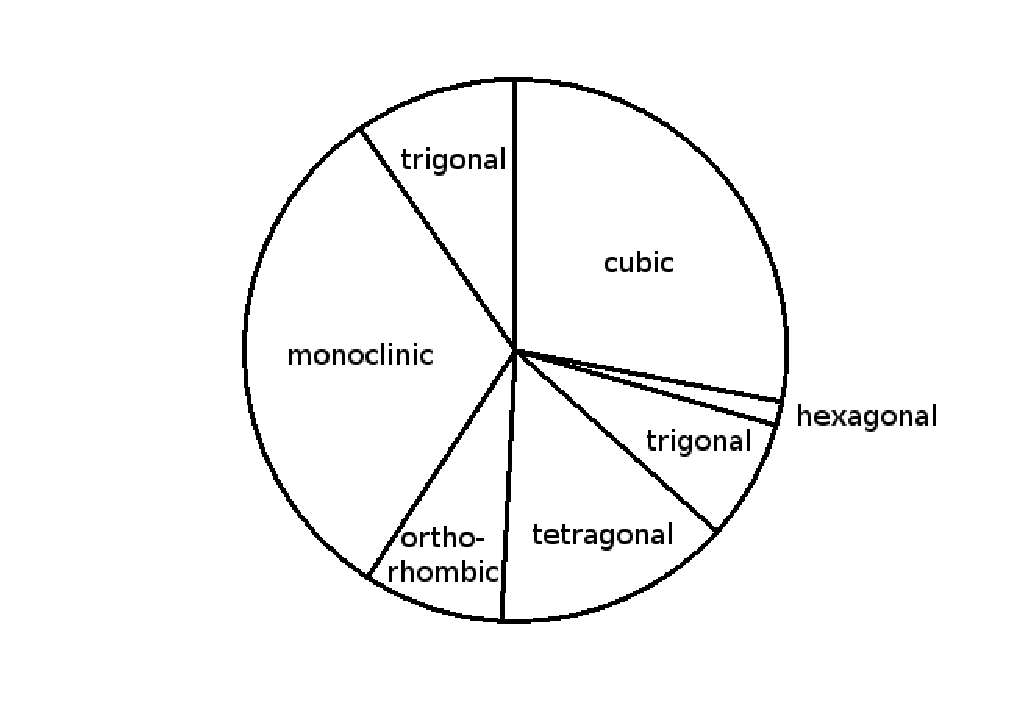
\includegraphics{crystalSystems.eps}}
%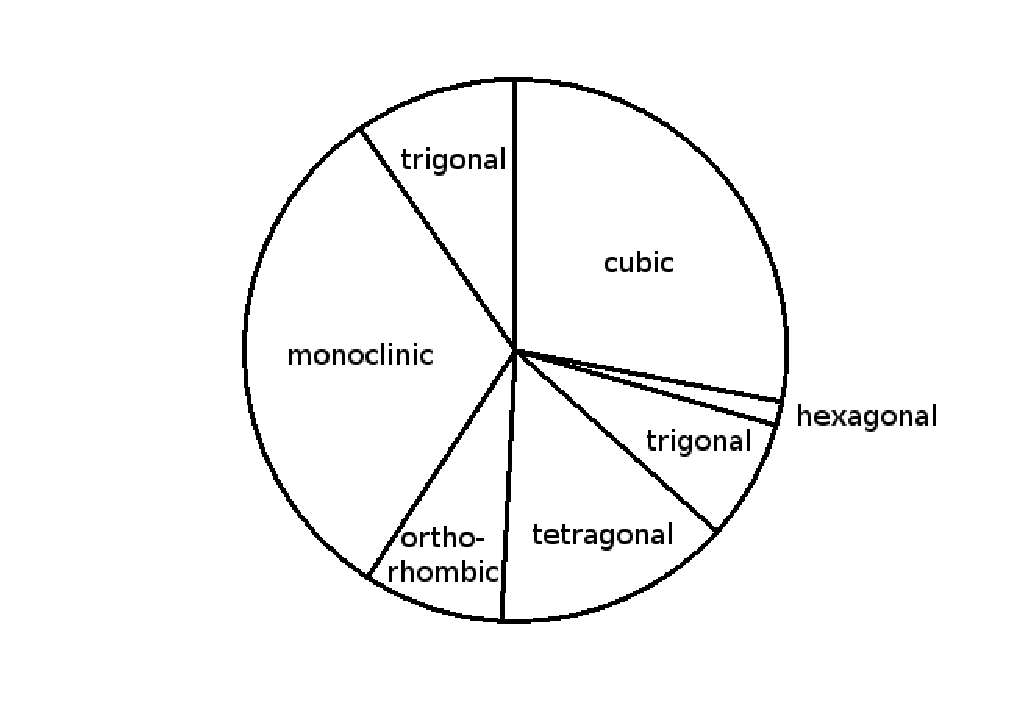
\includegraphics{crystalSystems.eps}
\caption[Distribution of experimental structures among the seven
crystal systems.]{Crystal systems for crystals of tetrahedral
molecules.\label{distro}}
\end{center}
\end{figure}

\begin{table}
\caption{Reference lattices for cubic (isometric) structures.}
\label{cubic}
\begin{center}
\begin{tabular}{cccc}%\hline
\cline{1-4}
Structure & Example & $|G|/Z$ & Entries \\
        & Lattice \\
\cline{1-4}
227a    & ZNOXAC01 & 24 & 1 \\
        & diam     & 24 \\
217a    & DEQPAQ   & 24 & 11 \\
        & bcc      & 48 \\
215a    & FOHCUA   & 24 & 3 \\
        & sc       & 48 \\
205c    & FOJBUB02 &  3 & 2 \\
        & d-fcc$^*$& 24 \\
218a,c  & SENLAY   &  3 & 3 \\
        & A15      &  6 \\
\cline{4-4}
\multicolumn{3}{r}{total:} & 20 \\
\cline{1-4}
\end{tabular} \\
$^*$ dimer packing
\end{center}
\end{table}

\begin{figure}
\begin{center}
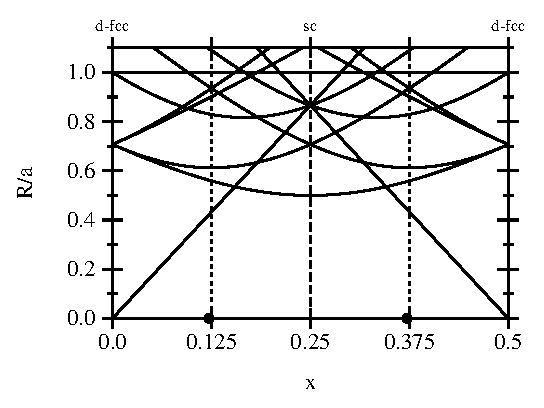
\includegraphics{205c.eps}
\end{center}
\caption[Neighbor distances for 205c as a function of $x$]{Neighbor
distances for 205c as a function of the Wyckoff structural
parameter, $x$.  The experimental structures, marked with circles,
are midway between the sc and doubly-occupied fcc limits.}
\label{fig:205c}
\end{figure}

\begin{figure}
\begin{center}
\scalebox{1}{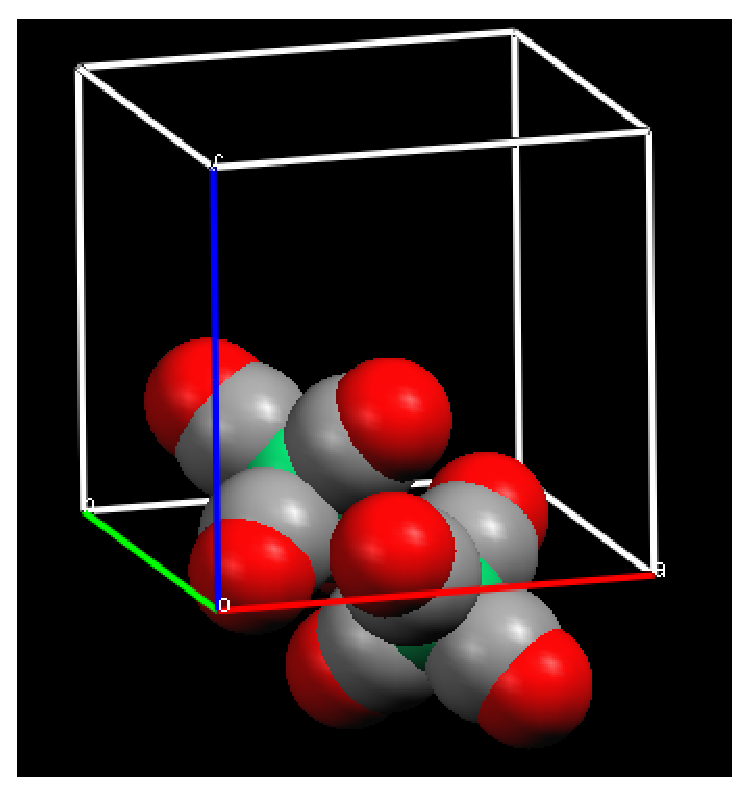
\includegraphics{FOJBUB02_Show.eps}}
%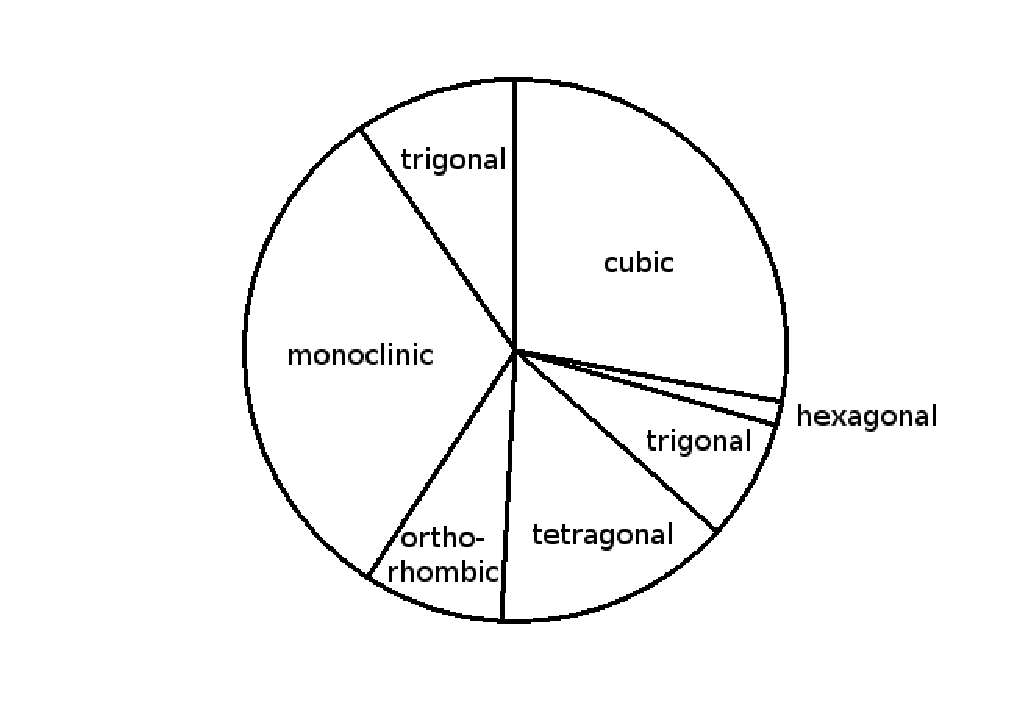
\includegraphics{crystalSystems.eps}
\caption[Crystal structure of tetracarbonyl-nickel in space group
205c]{Crystal structure of tetracarbonyl-nickel [CSD structure
FOJBUB02~\cite{Braga93}] in space group 205c with molecules at
Wyckoff point c. It is a fcc lattice of dimers at Wyckoff point a as
shown for one dimer centered at fractional coordinate
$(1/2,1/2,0)$.\label{dimers}}
\end{center}
\end{figure}

\begin{table}
\caption[Reference lattices for hexagonal and trigonal
structures.]{Reference lattices for hexagonal and trigonal
structures. Ideal reference lattice parameters and Wyckoff
structural parameters are listed below the experimental data.}
\label{hex}
\begin{center}
\begin{tabular}{cccccc}%\hline
\cline{1-6}
Structure & Example & c/a & Str.\ Param's & $|G|/Z$ & Entries \\
          & Lattice \\
\cline{1-6}
165d    & DILWIE01  & 3.07  & z=0.122          &  3 & 2 \\
        & hcp       & 3.27  & z=1/8            & 12 \\
161a    & TCYMET    & 1.28  & z=0.000          &  3 & 1 \\
        & bcc       & 1.22  & z=0              & 48 \\
147d    & ZIZHIZ    & 1.51  & z=0.252          &  3 & 1 \\
        & hcp       & 1.63  & z=1/4            & 12 \\
176h    & CUCZUV    & 0.89  & x=0.361, y=0.334 &  2 & 1 \\
        & hcp       & 0.94  & x=1/3, y=1/3     & 12 \\
152b    & MTRETC10  & 2.57  & x=0.715          &  2 & 1 \\
        & fcc       & 2.45  & x=2/3            & 48 \\
\cline{6-6}
\multicolumn{5}{r}{total:} & 6 \\
 \cline{1-6}
\end{tabular}
\end{center}
\end{table}

\begin{figure}
\begin{center}
\scalebox{1}{\includegraphics{tcymetSupercell_2.eps}} \caption[The
crystal structure of TCYMET embedded in a bcc reference
lattice.]{The crystal structure of TCYMET embedded in a bcc
reference lattice. The molecular centers of mass are depicted as
spheres. The lattice constant of the bcc reference lattice,
$a^\prime$, is compared to the lattice constants a and c of
TCYMET.\label{bccEmbed}}
\end{center}
\end{figure}

\begin{table}
\caption{Reference lattices for tetragonal structures} \label{tet}
\begin{center}
\begin{tabular}{cccccc}%\hline
\cline{1-6}
Structure & Example & c/a & Str.\ Parameters & $|G|/Z$ & Entries \\
          & Lattice \\
\cline{1-6}
141a    & FUZLUH    & 0.72 & & 8 & 2 \\
        & A5$^\prime$&0.76 & & 8 \\
137b    & FUZTEZ    & 0.70 & & 8 & 1 \\
        & Aa        & 0.82 & & 16 \\
121a    & ZZZKDW01  & 1.49 & & 8 & 1 \\
        & fcc       & 1.41 & & 48 \\
142a    & KUJSIR    & 2.02 & & 4 & 1 \\
        & fcc       & 2.00 & & 48 \\
120c    & YEMRIR    & 1.50 & & 4 & 1 \\
        & sc        & 1.41 & & 48 \\
114a    & ADAMAN08  & 1.34 & & 4 & 2 \\
        & fcc       & 1.41 & & 48 \\
88a     & KANGUB01  & 3.97 & & 4 & 1 \\
        & A5$^{\prime\prime}$& 3.46&&8 \\
88f     & LUFYEQ    & 1.25 & z=0.311&1&1 \\
        & d-Aa$*$     & 1.15 & z=3/8&8 \\
\cline{6-6}
\multicolumn{5}{r}{total:} & 10 \\
\cline{1-6}
\end{tabular} \\
$^*$ dimer packing
\end{center}
\end{table}

\begin{figure}
% \includegraphics{141ab.eps}
% \includegraphics{139ab.eps}
\begin{center}
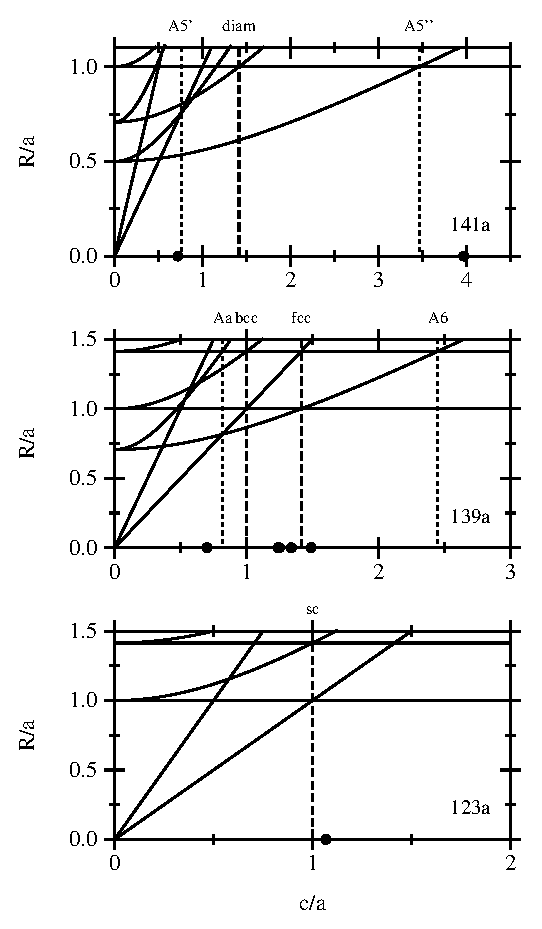
\includegraphics{tetrEPS.eps}
\end{center}
\caption[Neighbor distances for 141a, 139a, and 123a]{Neighbor
distances for 141a, 139a, and 123a as a function of the $c/a$ ratio.
The tetragonal distortions include diam, bcc, fcc, and sc as special
cases.  Experimental values are marked with circles.  Additional
neighbors are omitted for clarity at small $c/a$ values.}
\label{fig:tetr}
\end{figure}

\begin{table}
\caption{Reference lattices for orthorhombic structures}
\label{orth}
\begin{center}
\begin{tabular}{ccccccc}%\hline
\cline{1-7}
Structure & Example & b/a & c/a & Str.\ Parameters & $|G|/Z$ & Entries \\
          & Lattice \\
\cline{1-7}
62c     & GUTCED    & 1.10  & 1.09  & x=0.171, z=-0.014   & 2  & 1 \\
        & fcc       & 1.00  & 1.00  & x=1/4, z=0         & 48 \\
62c     & RIMMOP    & 1.46  & 1.61  & x=0.187, z=0.032   & 2  & 1 \\
        & bcc       & 1.41  & 1.41  & x=1/4, z=0         & 48 \\
62c     & JEYSEL    & 1.62  & 1.80  & x=-0.069, z=-0.030   & 2  & 1 \\
        & sh        & 1.63  & 1.73  & x=0, z=0           & 24 \\
64d,f   & METHANEIII& 0.70  & 0.70  & x=0.250            & 1  & 1 \\
        &           &       &       & y=0.230, z=0.270    \\
        & fcc       & 0.71  & 0.71  & x=1/4              & 48 \\
        &           &       &       & y=1/4, z=1/4 \\
19a     & MZNMOX10  & 1.03  & 3.93  & x=-0.066, y=0.067, z=0.123 & 1 & 1 \\
        & 63c       & 1.00  & 3.15  & x=0, y=0, z=0.112          & 4 \\
60c,d   & YIMWEW    & 0.45  & 0.46  & y=-0.188            & 2/3 & 1 \\
        &           &       &       & x=0.169, y=0.297, z=0.206 \\
        & bcc       & 0.47  & 0.47  & y=-1/4              & 48 & \\
        &           &       &       & x=1/6, y=1/4, z=1/4 \\
\cline{7-7}
\multicolumn{6}{r}{total:} & 6 \\
\cline{1-7}
\end{tabular}
\end{center}
\end{table}

\begin{table}
\caption{Reference lattices for monoclinic structures} \label{mono}
\begin{center}
\begin{tabular}{cccccccc}%\hline
\cline{1-8}
Structure & Example & b/a & c/a & $\beta$ & Str.\ Parameters & $|G|/Z$ & Entries \\
          & Lattice \\
\cline{1-8}
15e     & REKYUB    & 0.48 & 1.00 & 123 & y=-0.024 & 2 & 3 \\
        & fcc       & 0.58 & 1.16 & 125 & y=0   & 48 \\
15e     & RASDOE    & 0.51 & 0.97 & 120 & y=0.123 & 2 & 1 \\
        & 70a       & 0.50 & 1.00 & 120 & y=1/8   & 4 \\
15e     & TMGEHS10  & 1.78 & 1.14 & 108 & y=0.106 & 2 & 3 \\
        & A5$^\prime$& 1.87 & 1.06 & 118 & y=1/8   & 8 \\
12i     & MECKOU    & 0.73 & 1.17 & 110 & x=0.253, z=0.241 & 2 & 1 \\
        & fcc       & 0.58 & 1.00 & 109 & x=1/4, z=1/4     & 48 \\
11e     & MECKIO    & 1.61 & 1.13 & 105 & x=0.205, y=0.219 & 2 & 1 \\
        & bcc       & 1.63 & 1.00 & 109 & x=1/4, y=1/4     & 48 \\
14e     & TOHSUE    & 1.01 & 2.76 & 90  & x=0.250, y=0.745, z=0.126 & 1 & 1\\
        & fcc       & 1.00 & 2.83 & 90  & x=1/4, y=3/4, z=1/8       & 48 \\
14e     & TMSIAD    & 1.11 & 2.07 & 91  & & 1 & 1 \\
        & d-sh$*$  & 1.22 & 2.12 & 90  & & 12 \\
14e     & CAMPOV    & 1.41 & 1.64 & 92  & & 1 & 2 \\
        & d-sc$*$   & 1.41 & 1.41 & 90  & & 24 \\
14e     & DOCNIS    & 1.45 & 1.80 & 60  & x=0.102, y=0.255, z=0.072 & 1 & 1 \\
        & hcp       & 1.63 & 2.00 & 60  & x=1/6, y=1/4, z=1/12      & 12 \\
14e     & CARBTC    & 0.63 & 1.01 & 104 & x=0.248, y=0.067, z=0.157 & 1 & 1 \\
        & hcp       & 0.61 & 1.06 & 90  & x=1/4, y=0, z=1/6         & 12 \\
14e     & QUGBOJ    & 0.59 & 1.06 & 105 & x=0.268, y=0.129, z=0.070 & 1 & 1\\
        & A5$^\prime$&0.76 & 1.00 & 90  & x=1/4, y=1/8, z=0         & 8 \\
\cline{1-8}
\end{tabular}\\
$^*$ dimer packing
\end{center}
\end{table}

\begin{table}
\caption{cont.}
\begin{center}
\begin{tabular}{cccccccc}%\hline
\cline{1-8}
Structure & Example & b/a & c/a & $\beta$ & Str.\ Parameters & $|G|/Z$ & Entries \\
          & Lattice \\
\cline{1-8}
14e     & MECKUA    & 0.66 & 1.14 & 113 & x=0.501, y=0.225, z=0.749 & 1 & 1 \\
        & fcc       & 0.59 & 1.00 & 109 & x=1/2, y=1/4, z=3/4       & 48 \\
14e,e   & CANFIG    & 0.92 & 1.10 & 26  & x=0.331, y=0.340, z=0.005 & 1/2 & 1 \\
        & d-136$*$  & 1.00 & 1.12 & 27  & x=1/3, y=1/3, z=0         & 2 \\
14e,e   & MXSNOX    & 1.76 & 1.74 & 75  & & 1/2 & 1 \\
        & d-sh$*$   & 1.73 & 1.91 & 59  & & 12 \\
13e,f,g & RIMNAC    & 0.52 & 1.84 &  94 & y=0.480 & 1/2 & 1 \\
        &           &      &      &     & y=0.813 \\
        &           &      &      &     & x=0.256, y=0.158, z=0.001 \\
        & 70a       & 0.50 & 1.73 &  90 & y=3/8   & 4 \\
        &           &      &      &     & y=5/8 \\
        &           &      &      &     & x=1/4, y=1/8, z=0 \\
15f,f,f,f  & CTBROM & 0.57 & 0.98 & 111 & x=0.096, y=0.032, z=0.378 & 1/4 & 2 \\
        &           &      &      &     & x=0.379, y=0.060, z=0.120  \\
        &           &      &      &     & x=0.126, y=0.316, z=0.123  \\
        &           &      &      &     & x=0.345, y=0.291, z=0.371  \\
        & fcc       & 0.58 & 1.00 & 109 & x=1/8, y=0, z=3/8          & 48 \\
        &           &      &      &     & x=3/8, y=0, z=1/8  \\
        &           &      &      &     & x=1/8, y=1/4, z=1/8  \\
        &           &      &      &     & x=3/8, y=1/4, z=3/8  \\
\cline{8-8}
\multicolumn{7}{r}{total:} & 22 \\
\cline{1-8}
\end{tabular}\\
$^*$ dimer packing
\end{center}
\end{table}

\begin{table}
\caption{Reference lattices for triclinic structures} \label{tri}
\begin{center}
\begin{tabular}{cccccccccc}%\hline
\cline{1-10}
Structure & Example & b/a & c/a & $\alpha$ & $\beta$ & $\gamma$ & Str.\ Parameters & $|G|/Z$ & Entries \\
          & Lattice \\
\cline{1-10}
2i      & BASXOI    & 1.15 & 1.15 & 86 & 90 & 66 & x=0.297, y=0.306, z=0.299 & 1 & 1 \\
        & A6        & 1.00 & 1.00 & 90 & 90 & 60 & x=1/4, y=1/4, z=1/4       & 16 \\
2i      & XAGXAE    & 1.02 & 1.02 & 93 & 101 & 110 &                         & 1 & 1 \\
        & d-Ai$*$  & 1.15 & 0.83 & 87 & 97 & 116  &                         & 6 \\
2i      & XUWROW    &      &      &    &   &       &                         & & - \\
        & \multicolumn{9}{l}{epitaxial crystal---70\% voids} \\
2i      & MEZDIE01  & 1.46 & 0.92 & 90 & 112 & 90 & x=0.261, y=0.251, z=0.242 & 1 & 2\\
        & bcc       & 1.63 & 1.00 & 90 & 109 & 90 & x=3/4, y=1/4, z=1/4       & 48 \\
2i,i,i  & OHABEE    & 1.49 & 2.57 & 90 & 90 & 90 & x=0.320, y=0.247, z=0.585  & 1/3 & 1 \\
        &           &      &      &    &    &    & x=0.016, y=0.254, z=0.250 \\
        &           &      &      &    &    &    & x=0.318, y=0.754, z=0.082 \\
        & bcc       & 1.63 & 2.83 & 90 & 90 & 90 & x=1/3, y=1/4, z=7/12       & 48 \\
        &           &      &      &    &    &    & x=0, y=1/4, z=1/4 \\
        &           &      &      &    &    &    & x=1/3, y=3/4, z=1/12 \\
2i,i,i,i & CANFOM   & 0.92 & 0.48 & 88 & 91 & 88 & x=0.162, y=0.842, z=0.484  & 1/4 & 1\\
        &           &      &      &    &    &    & x=0.334, y=0.340, z=-0.008 \\
        & d-136$*$  & 1.00 & 0.50 & 90 & 90 & 90 & x=1/6, y=5/6, z=1/2        & 2 \\
        &           &      &      &    &    &    & x=1/3, y=1/3, z=0 \\
\cline{10-10}
\multicolumn{9}{r}{total:} & 7 \\
\cline{1-10}
\end{tabular}\\
$^*$ dimer packing
\end{center}
\end{table}

\begin{table}
\caption{Summary of reference lattices inferred from experimental
data.} \label{summary}\scriptsize
\begin{tabular}{cccccccccc}
\hline
Struktur- & Pearson & Common & Space & Wyckoff & $|G|/Z$ & Comments & Monomer & Dimer & Occurance\\
bericht & Symbol & Name & Group & Point(s) & & & Structures & Structures & Percentage\\
\hline
A2  & cI2 & bcc & 229 & a           & 48 & sphere packing                         & 18 &   & 25.7\%\\
A1  & cF4 & fcc & 225 & a or b      & 48 & sphere packing                         & 15 & 2 & 24.3\%\\
Ah  & cP1 & sc  & 221 & a or b      & 48 & sphere packing                         &  4 & 2 & 8.6\%\\
A3  & hP2 & hcp & 194 & c or d      & 12 & sphere packing                         &  6 &   & 8.6\%\\
A5$^\prime$ & tI4 & & 141 & a or b  &  8 & distorted diamond with c/a=$2/\sqrt 7$ &  6 &   & 8.6\%\\
Af  & hP1 & sh  & 191 & a           & 24 & simple hexagonal                       &  1 & 2 & 4.3\%\\
A15 & cP8 &     & 223 & a and (c or d)&6 & least-area structure                   &  3 &   & 4.3\%\\
Aa  & tI2 & bct & 139 & a or b      & 16 & distorted bcc with c/a=$\sqrt 2/3$    &  1 & 1 & 2.9\%\\
    & tP8 &     & 136 & f,f         &  8 & dimer packing                          &    & 2 & 2.9\%\\
    & oF8 &     & 70  & a           &  4 &                                        &  2 &   & 2.9\%\\
A4  & cF8 & diamond & 227 & a or b  & 24 & sphere packing                         &  1 &   & 1.4\%\\
Ai  & tR2 &     & 166 & a,a         & 18 & dimer packing                          &    & 1 & 1.4\%\\
A6  & tI2 & fct & 139 & a or b      & 16 & distorted fcc with c/a=$\sqrt 6$       &  1 &   & 1.4\%\\
A5$^{\prime\prime}$ & tI4 & & 141 & a or b  & 8 & distorted diamond with c/a=$2\sqrt 3$&1& & 1.4\%\\
    & oC2 &     &  63 & c           &  8 &                                        &  1 &   & 1.4\%\\
\hline
\end{tabular}
\end{table}

\begin{figure}
\begin{center}
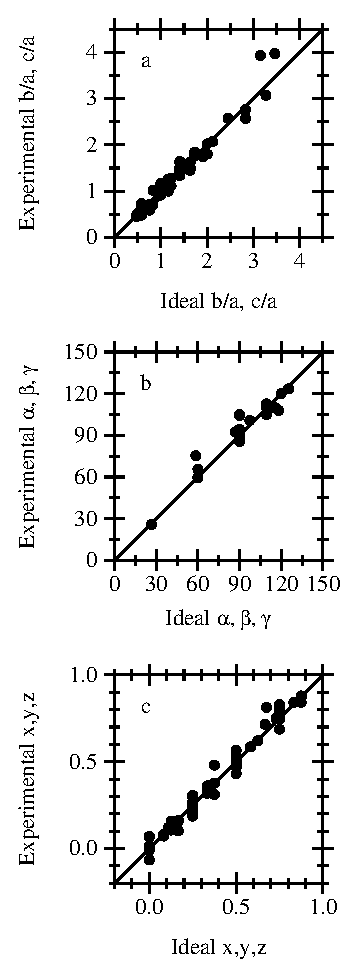
\includegraphics{compare2EPS.eps}
\end{center}
\caption[Comparison of experimental and ideal reference
structures.]{Comparison of experimental and ideal reference (a)
lattice lengths, (b) angles, and (c) structural parameters. The
45-degree line indicates perfect agreement between the experimental
molecular centers and the reference lattice. Scatter around the line
is the result of broken symmetry in orientationally ordered
structures.} \label{comparison}
\end{figure}

\begin{figure}
\begin{center}
\scalebox{.60}{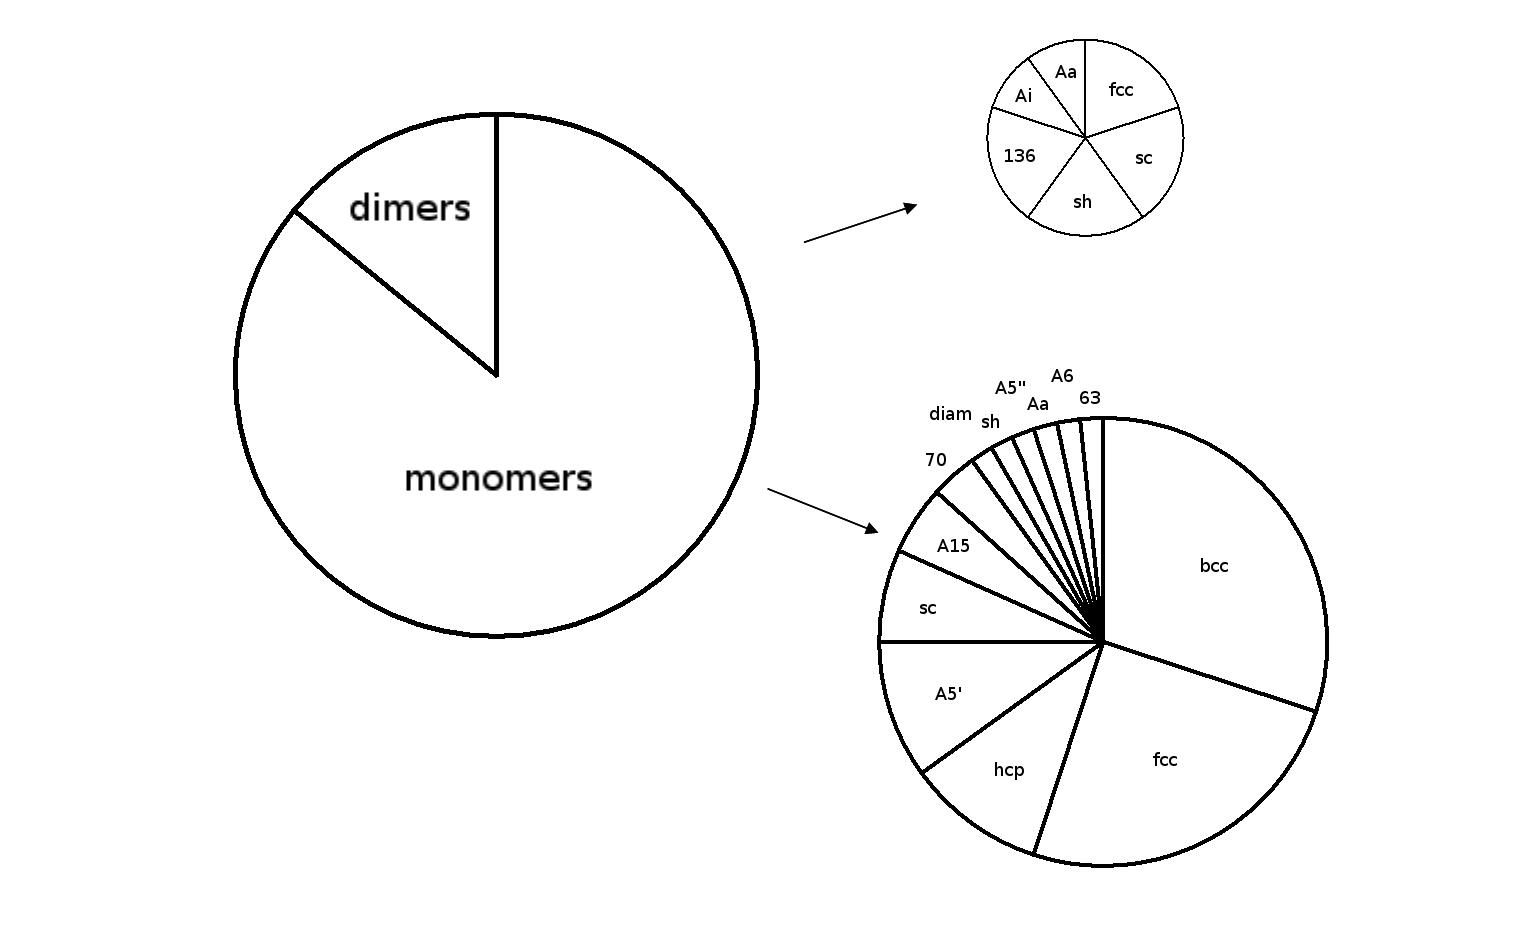
\includegraphics{pieCharts3.eps}}
\end{center}
\caption[Monomer and dimer structures and their reference
lattices.]{Relative proportions of monomer and dimer structures in
the experimental data set and reference lattices for
each.}\label{dimerMonomer}
\end{figure}

\begin{table}
\begin{center}
\caption{Dimer complexes among crystals of tetrahedral
molecules.}\label{tab:dimers}
\begin{tabular}{lccccc}
\hline
structure & dimer & representative & reference & point-group & entries\\
          &Wyck.~Pt.& entry        & lattice   & symmetry \\
\hline
205c & a & FOJBUB02 & d-fcc & $D_{3d}$              & 2\\
88f  & e & LUFYEQ   & d-Aa  & $C_{2v}$              & 1\\
14e  & a & TMSIAD   & d-sh  & $C_i$ ($\sim D_{3d}$) & 1 \\
14e  & a & CAMPOV   & d-sc  & $C_i$ ($\sim D_{3d}$) & 2\\
14e,e& e & CANFIG   & d-136 & $C_1$ ($\sim D_{3d}$) & 1\\
14e,e&b,c& MXSNOX   & d-sh  & $C_i$ ($\sim D_{3d}$) & 1\\
2i   & a & XAGXAE   & d-166 & $D_{3d}$              & 1\\
2i,i,i,i&i,i&CANFOM & d-136 & $C_1$ ($\sim D_{3d}$) & 1 \\
\cline{6-6}
\multicolumn{5}{r}{total:} & 10 \\
\hline \multicolumn{6}{c}{{\small Note: Point group symmetries were
assigned by visual inspection.}}
\end{tabular}
\end{center}
\end{table}

\bibliography{thesisbib}

\end{document}
